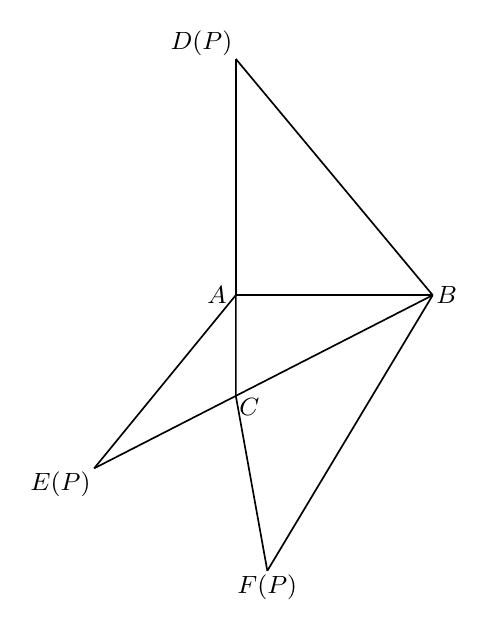
\begin{tikzpicture}[line width=0.6pt, font=\small]
% Plane unfolding of P-ABC: AB common edge, D/A/F vertical, EB crosses AF at C
\coordinate (A) at (0,1.0);
\coordinate (B) at (2.5,1.0);
\coordinate (Dv) at (0,4.0);
\coordinate (E) at (-1.8,-1.2);
\coordinate (F) at (0.4,-2.5);
\coordinate (C) at (0,-0.28);
% upper triangle D-A-B
\draw (Dv) -- (A);
\draw (Dv) -- (B);
\draw (A) -- (B);
% lower-left triangle A-E-B
\draw (A) -- (E);
\draw (E) -- (B);
% lower segment A-C-F and B-F
\draw (A)--(C)--(F);
\draw (B) -- (F);
% labels
\node[inner sep=1pt,above left] at (Dv) {$D(P)$};
\node[inner sep=1pt,left,fill=none,xshift=-2.00bp,yshift=0.00bp] at (A) {$A$};
\node[inner sep=1pt,right] at (B) {$B$};
\node[inner sep=1pt,below left] at (E) {$E(P)$};
\node[inner sep=1pt,below] at (F) {$F(P)$};
\node[inner sep=1pt,right,fill=none,xshift=0.00bp,yshift=-4.00bp] at (C) {$C$};
\end{tikzpicture}
